\section{Konzeption}
Nachdem nun die Grundlagen über die essenziellen Themen dieser Arbeit erläutert wurden, kann mit der Konzeption begonnen werden. Hier wird ein Überblick über die Planung des Vorgehens zur Zielerfüllung gegeben. Dabei soll zuerst eingegrenzt werden, was die Aufgabenstellung beinhaltet. Danach können Vorbereitungen getroffen werden, um das Protokoll in die Software des Tankautomaten zu integrieren. Auf dieser Basis dann ein finales Vorgehen erstellt werden.
\subsection{Aufgabenstellung}
Zuerst soll, mit Hilfe einiger getroffener Annahmen, die Aufgabenstellung eingegrenzt werden. Dies erleichtert nicht nur die Planung, da einige Szenarien damit außer Frage stehen, sondern diktiert auch weitere Dinge, die bei der Umsetzungsplanung berücksichtigt werden müssen. Im Folgenden werden diese Eingrenzungen und Randbedingungen vorgestellt.
%Um zu erarbeiten, wie die spätere Umsetzung realisiert werden kann, muss zuerst die Aufgabenstellung abgegrenzt werden. Zur bereits erklärten Aufgabenstellung wurden vom Auftragsgeber Einschränkungen, sowie Anforderungen vorgegeben, die in der Umsetzung beachtet werden mussten. Im Folgenden sollen diese Randbedingungen präsentiert und die Anforderungen aufgezeigt werden. 

\subsubsection{Randbedingungen}
Um den Umfang einzugrenzen, wurden zusätzlich zum Ziel einige Annahmen getroffen. Diese beziehen sich auf den Netzwerkaufbau, die Konfiguration der Ladesäulen und wie diese identifiziert werden können.\\

\noindent Bei der Planung wurde davon ausgegangen, dass die Ladesäulen entweder direkt über einen Local Proxy oder über ein \acfi{VPN} indirekt mit dem Tankautomaten Netzwerk verbunden sind. Außerdem wurde festgelegt, dass der Tankautomat als \ac{CSMS} agiert und die Ladesäulen sich als Clients mit diesem verbinden. Dieser Aufbau wurde in \autoref{fig:Tankautomaten_Netzwerk} zusätzlich mit dem Cloudserver und den genutzten Protokollen dargestellt.

\begin{figure}[H]
	\centering
	\includegraphics[width=0.8\textwidth]{images/OCPP/Topologie_Ladesäulen.png}
	\caption{Erwarteter Aufbau des Tankautomaten Netzwerks\cite{Eigene_Darstellung}}
	\label{fig:Tankautomaten_Netzwerk}
\end{figure}

\noindent Dabei sind die Ladesäulen so konfiguriert, dass der Verbindungsaufbau reibungslos stattfinden kann. Dies bezieht sich auf Einstellungen wie die IP-Adresse, den Port, die \acs{OCPP} Version und die Art der Kommunikationsverschlüsselung bzw. das OCPP Security Profile. Zudem ist bereits festgelegt, dass jeder Ladevorgang ausschließlich vom Tankautomaten gestartet wird und nur die Ladesäule diesen beendet. Hierfür wird ein Ladevorgang als beendet angesehen, sobald das Fahrzeug vollgeladen ist oder es ausgesteckt wurde.\\

\noindent Um dabei Ladesäulen von anderen Stationen wie z. B. den Zapfsäulen unterscheiden zu können, wurde die Cloud Weboberfläche und somit auch die lokale Datenbank mit zusätzlichen Feldern erweitert. Diese waren anfangs nicht genauer spezifiziert und wurden im Zuge der Konzeption erarbeitet (siehe \autoref{Cloud_Erweiterung}). Dabei ist die Anzahl an Feldern, die Bezeichnung und der Datentyp frei wählbar. Es wurde allerdings bereits festgelegt, dass die jeweilige OCPP Version der Ladesäule in dem bereits erwähntem Feld \glqq{}type\grqq{}, angegeben wird. Somit soll das Feld also um die beiden Werte: \glqq{}OCPP1.6\grqq{} und \glqq{}OCPP2.0.1\grqq{} erweitert werden.

\subsubsection{Anforderungen}
Da nun klar ist, von welchen Annahmen ausgegangen wurde, kann erläutert werden, welche Anforderungen der Kunde an die Erweiterung gestellt hat. Sie können dabei grob in die Kategorien: Terminal, Cloud-Schnittstelle und OCPP eingeordnet werden. Alle Anforderungen erhalten hierbei eine \acs{ID}. Diese ID dient der Übersichtlichkeit, damit in späteren Kapiteln eindeutig ist, auf welche Anforderung sich bezogen wurde.\\ \\
\noindent\textbf{Terminal Anforderungen}\newline
\noindent Die Anforderungen dieser Kategorie beziehen sich auf alle Funktionalitäten, die den Tankautomaten direkt betreffen. Dazu gehören die Anzeigen auf dem Display sowie die Freigaben und die Produktauswahl.
\begin{description}[leftmargin=34pt]
	\item[\textbf{T-01}] Die Berechtigung für den Fahrer, das Fahrzeug und die daraus resultierende Produktauswahl, erfolgt weiterhin wie bei den anderen Stationstypen.
	\item[\textbf{T-02}] Wenn min. eine oder mehrere Stationen mit dem Typ \glqq{}OCPP1.6\grqq{} oder \\
	\glqq{}OCPP2.0.1\grqq{} konfiguriert sind, werden diese in der Produktauswahl auf dem Terminal angezeigt.
	\item[\textbf{T-03}] Wird in der Produktauswahl eine E-Ladesäule ausgewählt, öffnet sich eine neue Anzeige mit einer zusätzlichen Zahleneingabe.
	\item[\textbf{T-04}] Über die eingegebene Nummer wird die Ladesäule identifiziert.
	\item[\textbf{T-05}] Sollte die Ladesäule nicht existieren, belegt sein, der Fahrer für diese nicht berechtigt oder kein Fahrzeug angeschlossen sein, sollte eine Fehlermeldung angezeigt werden.
	\item[\textbf{T-06}] Wenn keine Fehler bei der Nummerneingabe auftraten, wird ein Ladevorgang an der Ladesäule gestartet.
	\item[\textbf{T-07}] Nachdem ein neuer Ladevorgang gestartet wurde, wird dieser in einer Übersicht mit den restlichen aktiven Tankvorgängen angezeigt.
	\item[\textbf{T-08}] In dieser Übersicht wird die aktuelle Lademenge in kWh angezeigt.
	\item[\textbf{T-09}] Nachdem ein Ladevorgang von der Ladesäule beendet wurde, ist dieser noch für 60s in der Übersicht zu sehen und wird danach entfernt.
\end{description}

\noindent\textbf{Cloud-Schnittstellen Anforderungen}\\
Alle Anforderungen, die sich auf die Cloud-API beziehen, beinhalten den Datenaustausch zwischen dem Tankautomaten und dem Cloudserver.
\begin{itemize}[leftmargin=38pt]
	\item[\textbf{C-01}] Der Verbindungsstatus pro Ladesäule wird in einem 60s Intervall an den Cloudserver gesendet. Dieser kann in der Weboberfläche eingesehen werden.
	\item[\textbf{C-02}] Wird ein Ladevorgang beendet, werden die Transaktionsdaten (Fahrer, Fahrzeug, Lademenge etc.) an den Cloudserver gesendet.
\end{itemize}

\noindent\textbf{OCPP Anforderungen}\\
Als Letztes gibt es die OCPP Anforderungen. Diese beziehen sich auf den gewünschten Funktionsumfang des Protokolls.
\begin{itemize}[leftmargin=38pt]
	\item[\textbf{O-01}] Dem Tankautomat muss es möglich sein, einen Ladevorgang an der Ladesäule zu starten.
	\item[\textbf{O-02}] Während eines Ladevorgangs muss in einem regelmäßigen Abstand die Lademenge übertragen werden.
	\item[\textbf{O-03}] Das Terminal muss erkennen, falls ein Ladevorgang durch die Ladesäule beendet wurde.
\end{itemize}

\noindent Für die OCPP Anforderungen gilt zusätzlich, dass alle gelisteten Funktionalitäten, für beide Versionen implementiert werden müssen. Alle Anforderungen beschreiben das Ziel der Erweiterung und sollen später anhand von Tests auf ihre Erfüllung überprüft werden (siehe \autoref{Test_Kapitel}).

\subsection{Benötigte OCPP Funktionalität}
Die eben genannten Anforderungen für den Tankautomaten und die Cloud Schnittstelle sind ausreichend präzise, jedoch sind die Anforderung an das OCPP Protokoll nicht präzise genug um die Erweiterung planen zu können. Deswegen musste zuerst analysiert werden, welche Nachrichten des OCPP Protokolls benötigt werden, um die Anforderungen O-01 bis O-03 zu erfüllen.

\subsubsection{Allgemein}
Das OCPP Protokoll ist in der Version 1.6 dafür ausgelegt, in einem gewissen Umfang implementiert zu werden. In OCPP1.6 sollte eine komplette Gruppe an Features, ein sog. Feature Profile, implementiert werden (vgl. \cite{OCPP-1.6-edition-2}, S.9). OCPP2.0.1 hat diese Vorgabe nicht, weshalb unklarer ist, welche Features benötigt werden (vgl. \cite{OCPP-2.0.1-part0-introduction}, S.12). Da allerdings nur sehr wenige Funktionen des Protokolls überhaupt zur Steuerung benötigt werden und eine komplette Integration des Protokolls unwirtschaftlich, zeitaufwendig und unnötig ist, muss der Umfang eingegrenzt werden.  Um herauszufinden, welche OCPP Nachrichten benötigt werden, musste betrachtet werden, wie ein OCPP konformer Ablauf für die hier anfallenden \textit{use-cases} aussieht. Daher wurde auf Basis der OCPP Dokumentation, die Abfolgen der unterschiedlichen Transaktionen modelliert. 
\noindent Zur besseren Übersicht wurden die Abläufe aufgeteilt in drei Kategorien und ihre \textit{use-cases}: 
\begin{enumerate}
	\item \textbf{Boot Phase}: Verhalten der Ladesäule bei erstmaliger Verbindung mit dem \acs{CSMS} und Aufrechterhaltung der Verbindung.
	\item \textbf{Start eines Ladevorgangs}: Starten der Transaktion ausgehend vom \acs{CSMS} und Übertragung der Lademenge während der Transaktion.
	\item \textbf{Stopp eines Ladevorgangs}: Stopp einer gestarteten Transaktion, ausgehend von der Ladesäule
\end{enumerate}
Die einzelnen Abläufe der Phasen sollen nun anhand von Ablaufdiagrammen grafisch abgebildet werden.
Dabei sind die gezeigten beispielhaften Abläufe mit den Nachrichtentypen der OCPP Version 1.6 dargestellt. Die äquivalenten Abläufe für die Version 2.0.1 sind im \autoref{Ablauefe_OCPP201} zu finden.

\subsubsection{Boot Phase}
Nachdem erfolgreich eine WebSocket Verbindung nach \autoref{WebSockets} zwischen dem Tankautomaten und einer Ladesäule eröffnet wurde, findet der Bootvorgang statt. Dieser ist in \autoref{fig:Boot_Pending} zusehen. Die durchgehenden Pfeile bezeichnen hier immer eine Anfrage (\textit{request, kurz: req}) und die gestrichelten Pfeile eine Antwort (\textit{confirmation, kurz: conf}). Aus Gründen der Übersichtlichkeit wurden hier und in zukünftigen Ablaufdiagrammen, die Parameter bzw. der Payload der Nachrichten nur angegeben, falls diese wichtig für den Ablauf sind. 
\begin{figure}[H]
	\centering
	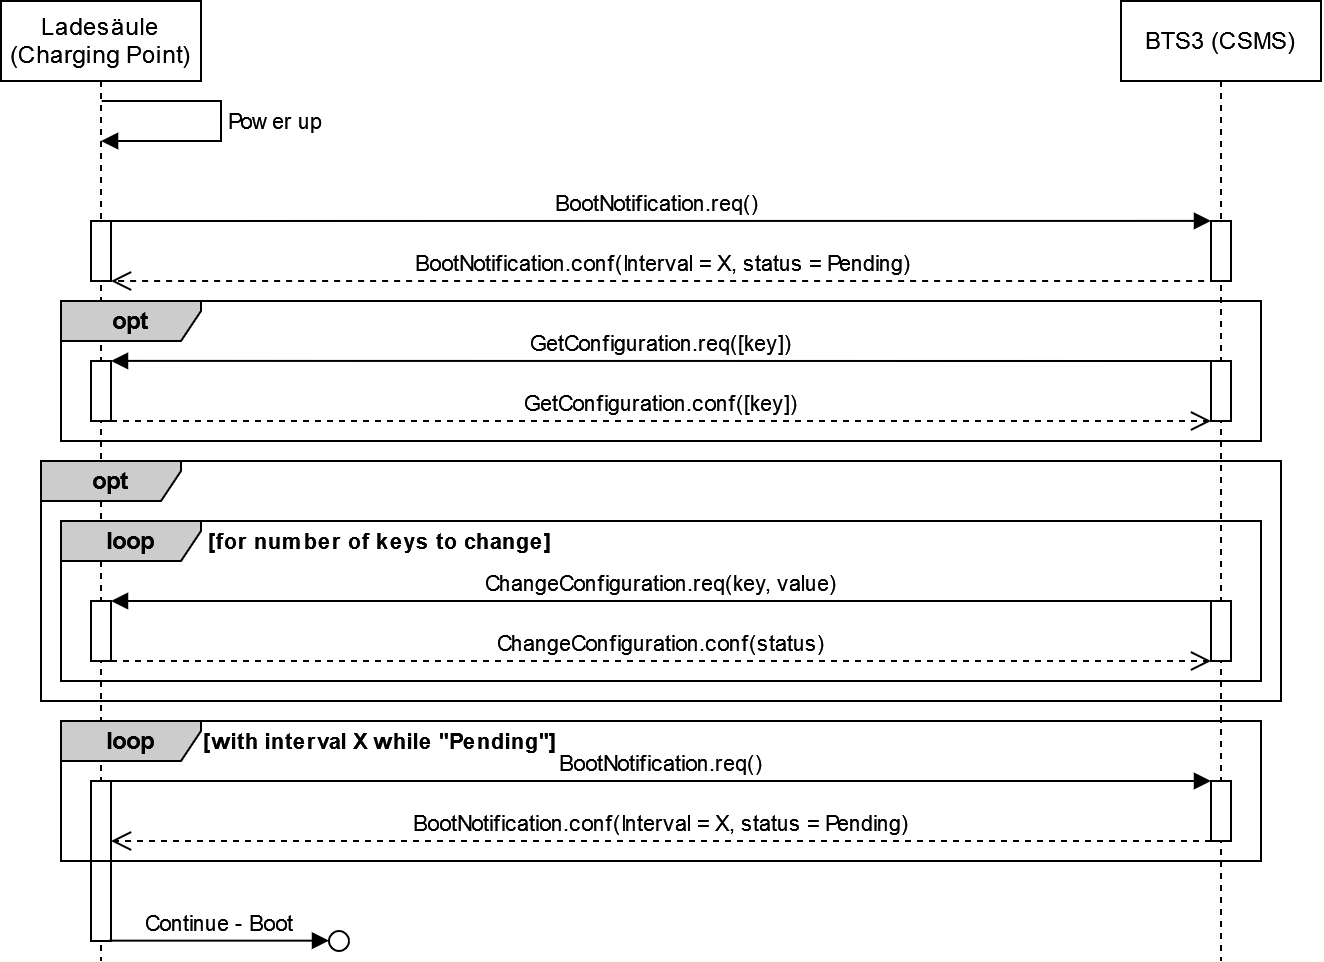
\includegraphics[width=1.0\textwidth]{images/OCPP/Boot_OCPP_v16.drawio.png}
	\caption{Ablauf Boot Pending mit Nachrichten Namen aus OCPP 1.6 \cite{Eigene_Darstellung, OCPP-1.6-edition-2}}
	\label{fig:Boot_Pending}
\end{figure}
\noindent Als erste Nachricht sendet die Ladesäule eine \spverb|BootNotification|, um sich beim \acs{CSMS} anzumelden. Das \acs{CSMS} antwortet darauf mit einem Intervall und einem Status. Der Status kann insgesamt drei Werte annehmen: 
\textit{Accepted}, \textit{Pending} und \textit{Rejected}. Solange mit einem Pending geantwortet wird, meldet sich die Ladesäule mit einem Intervall X beim \acs{CSMS}, bis entweder mit einem Rejected oder Accepted geantwortet wird. Während die Ladesäule auf ein Accepted wartet, kann das \acs{CSMS} mit einer \spverb|GetConfiguration| Nachricht, Konfigurationsparameter der Ladesäule abfragen. Diese werden als Liste an sie gesendet. Sollte das \acs{CSMS} einen Parameter ändern wollen, muss jeder Parameter einzeln mit einer \spverb|ChangeConfiguration| Nachricht geändert werden. \newline

\noindent Dabei sollten die Konfigurationsparameter: 
\spverb|StopTransactionOnEVDisconnect|, \\ \spverb|MetervalueSampledData|, \spverb|MetervalueSampleInterval| und \spverb|AuthorizeRemoteTx- Requests| richtig konfiguriert werden, da diese den Transaktionsablauf und die dabei übermittelten Daten beeinflussen können. Es kann allerdings nicht davon ausgegangen werden, dass alle diese Parameter veränderbar sind. Dies hängt von der Ladesäulen Implementierung ab (vgl. \cite{OCPP-1.6-edition-2}, S.46 \& \cite{OCPP-2.0.1-part2-specification-edition2}, S.53). Ebenfalls kann es sein, dass nach einer Parameteränderung die Ladesäule neu gestartet werden muss. Dies kann mit dem Befehl \verb|Reset| erfolgen.

\begin{figure}[H]
	\centering
	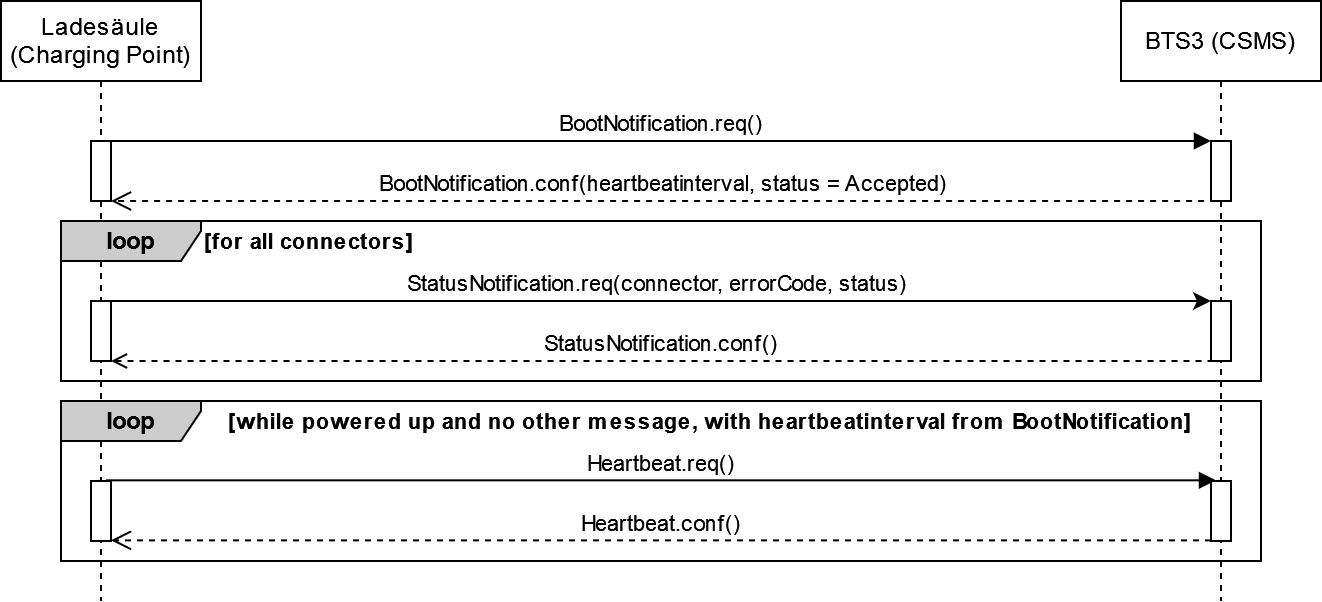
\includegraphics[width=1.0\textwidth]{images/OCPP/Boot_Success_16.drawio.png}
	\caption{Ablauf Boot Accepted mit Nachrichten Namen aus OCPP1.6 \cite{Eigene_Darstellung, OCPP-1.6-edition-2}}
	\label{fig:Boot_Succes_16}
\end{figure}

\noindent Sobald die Bootanfrage mit dem Status Accepted angenommen wurde, findet der Ablauf in \autoref{fig:Boot_Succes_16} statt. Hier teilt die Ladesäule dem \acs{CSMS} den aktuellen Status jedes Anschlusses mit. Neben dem Status wird ebenfalls ein \verb|errorCode| mit gesendet, der die aktuellen Störungen des Anschlusses meldet. Solange nun keine andere Nachricht gesendet wird und die Ladesäule nicht abgeschaltet wird, sendet sie im Intervall X eine \spverb|Heartbeat| Nachricht.

\begin{figure}[H]
	\centering
	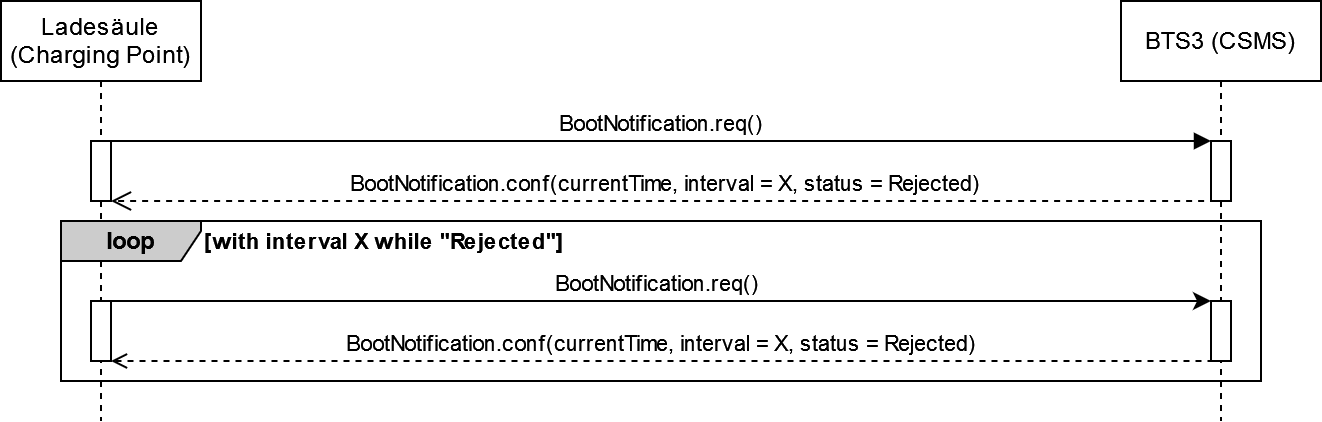
\includegraphics[width=1.0\textwidth]{images/OCPP/Boot_Rejected_16.drawio.png}
	\caption{Ablauf Boot Rejected mit Nachrichten Namen aus OCPP1.6 \cite{Eigene_Darstellung, OCPP-1.6-edition-2}}
	\label{fig:Boot_Rejected_16}
\end{figure}

\noindent Solange das \acs{CSMS} mit einem Status Rejected auf die \spverb|BootNotification| antwortet, wird weiterhin im Intervall X eine neue gesendet (siehe \autoref{fig:Boot_Rejected_16}).
\subsubsection{Start des Ladevorgangs}
Der Ladevorgang beginnt, wie in \autoref{fig:Start_Transaction_16} dargestellt, nachdem der Fahrer sein Fahrzeug an einer Ladesäule einsteckt. Dadurch wird der Status des Anschlusses auf \textit{Preparing} gesetzt. Der Fahrer wählt daraufhin die entsprechende Ladesäule aus und das \acs{CSMS} startet den Ladevorgang mit der \spverb|RemoteStartTransaction| Nachricht. Hier spielt der Konfigurationsparameter  \spverb|AuthorizeRemoteTxRequests| eine Rolle. Steht diese auf \textit{false} wird der Ladevorgang sofort mit einer\spverb|StartTransaction| Nachricht gestartet. Steht er auf \textit{true} wird zuerst mit einer \spverb|Authorize| Nachricht abgefragt, ob der mitgesendete \spverb|IdTag| zum Laden berechtigt ist. Nach der Bestätigung aktualisiert die Ladesäule den Status des Anschlusses auf \textit{Charging}. Während der Ladevorgang läuft, wird nun im Intervall: \spverb|MetervalueSampleInterval| ein Messwert, der in \spverb|MeterValueSampledData| angegeben wurde, an das \acs{CSMS} übertragen.
\begin{figure}[H]
	\centering
	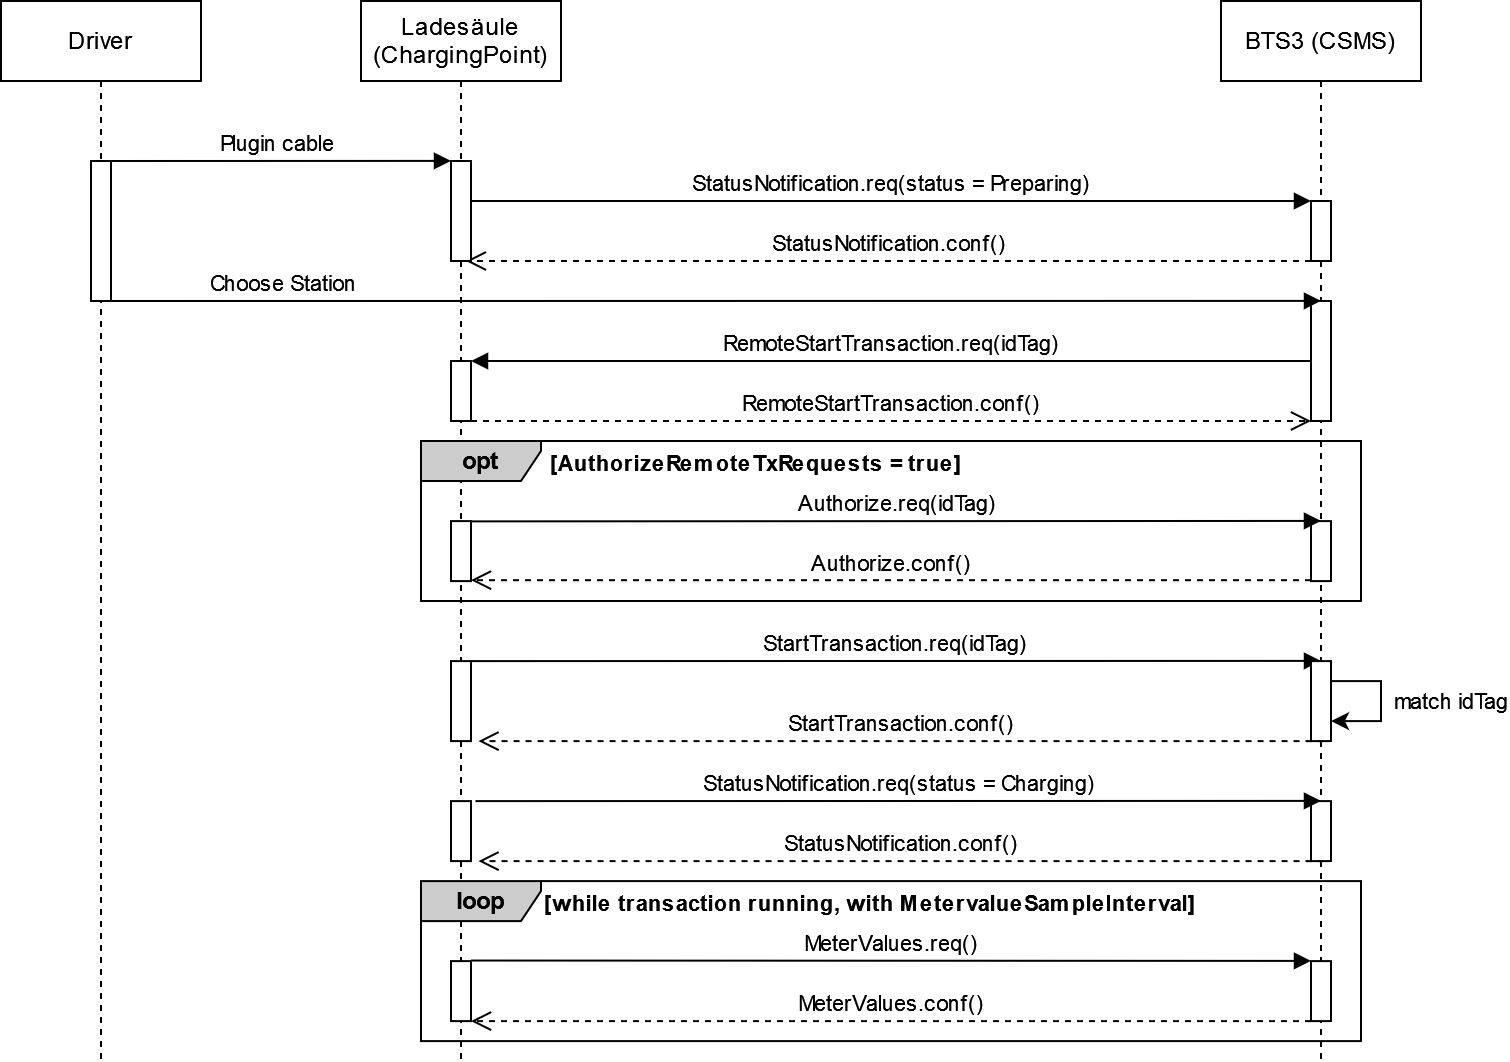
\includegraphics[width=0.9\textwidth]{images/OCPP/Charging_Start_OCPP_v16.drawio.png}
	\caption{Ablauf Ladevorgang Start mit Nachrichten Namen aus OCPP1.6 \cite{Eigene_Darstellung, OCPP-1.6-edition-2}}
	\label{fig:Start_Transaction_16}
\end{figure}

\subsubsection{Stopp des Ladevorgangs}
In \autoref{fig:Stopp_Transaction_16} ist der Stopp eines Ladevorgangs zu sehen. Damit der Ladevorgang wie in den Randbedingungen beschrieben durch das Ausstecken des Fahrzeuges beendet wird muss \verb|StopTransactionOnEVDisconnect| auf \textit{true} gesetzt sein. Ist das der Fall, sendet die Ladesäule eine \verb|StopTransaction| Nachricht nach dem Ausstecken des Fahrzeuges und ändert den Status zu \textit{Finishing}.
Falls das Kabel fest an der Ladesäule befestigt ist und nur auf der Fahrzeugseite ausgesteckt werden kann, wird direkt in den Status \textit{Available} gewechselt. Andernfalls wird der Status erst auf Available gesetzt, sobald das Kabel ebenfalls auf der Ladesäulen Seite ausgesteckt wurde. \\
\noindent Optional wird das Fahrzeug nicht mehr geladen, sobald es vollgeladen ist oder die Batterie zu heiß wird. Dabei wird der Status der Ladesäule auf \textit{SuspendedEV} gesetzt. Dies hat allerdings keinen Einfluss auf den danach folgenden Verlauf.
\begin{figure}[H]
	\centering
	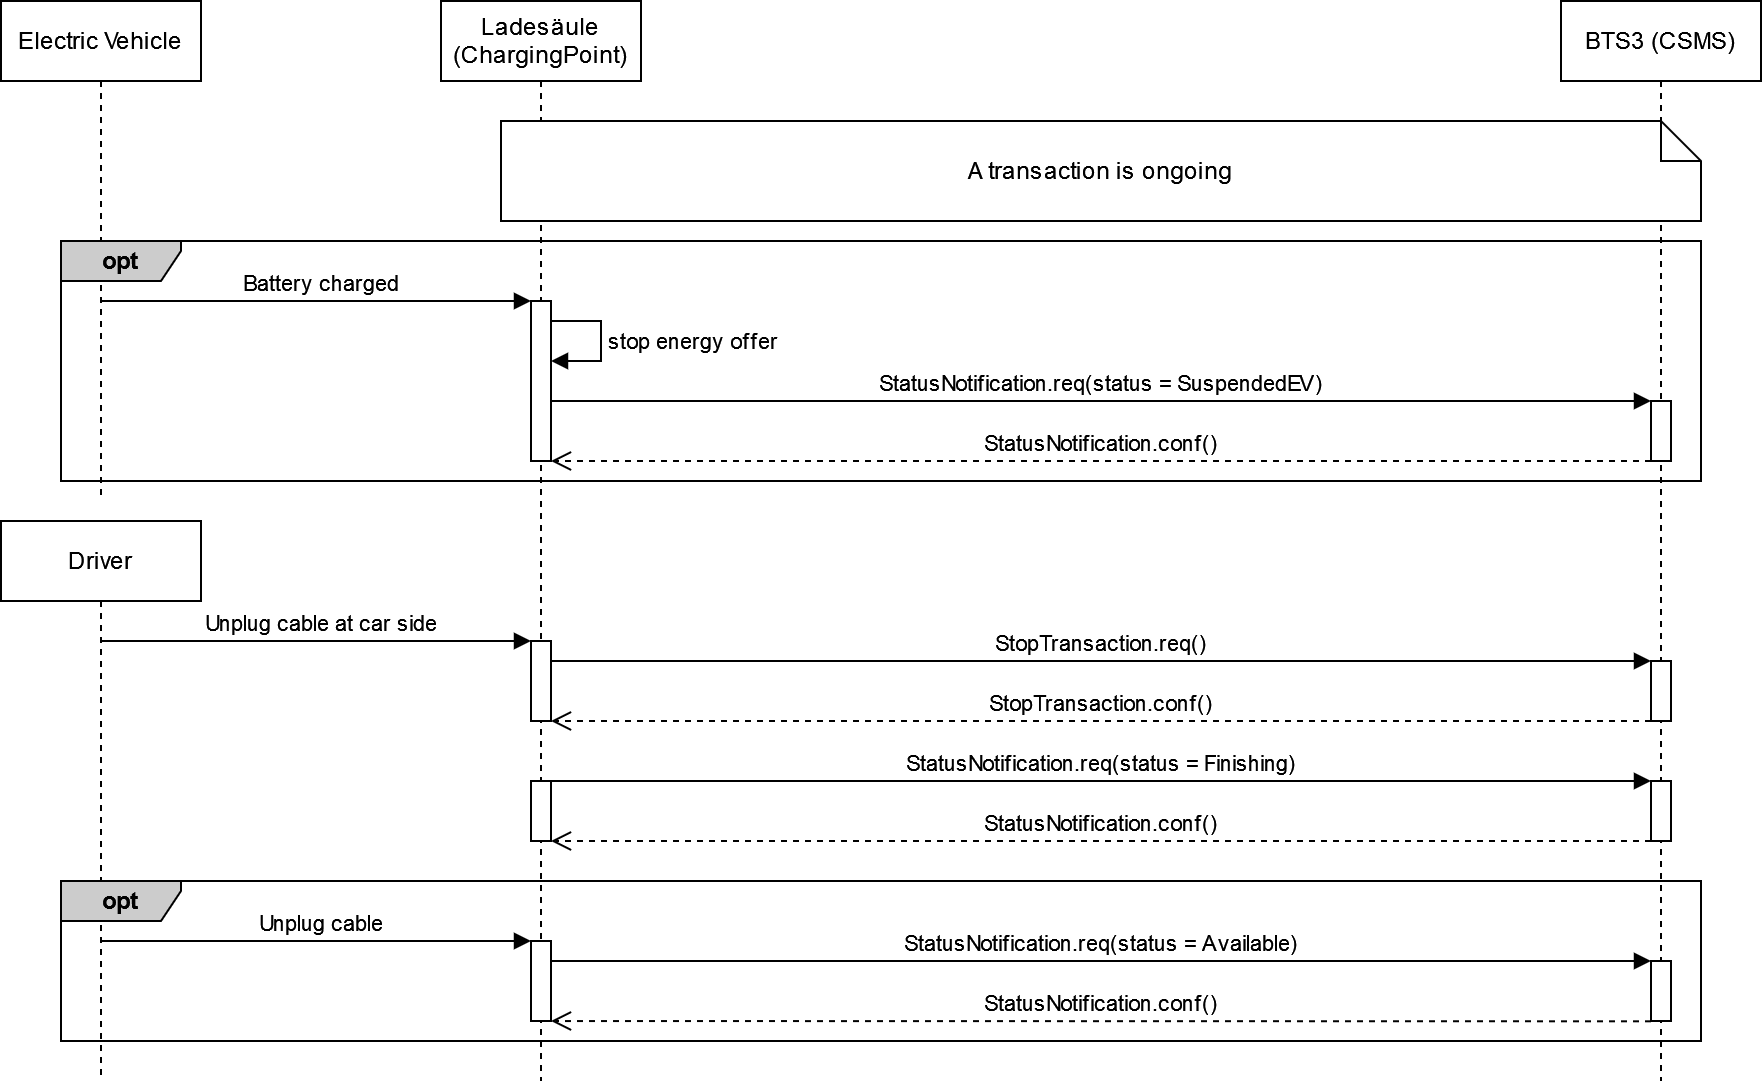
\includegraphics[width=1.0\textwidth]{images/OCPP/Charging_stop_OCPP_v16.drawio.png}
	\caption{Ablauf Ladevorgang Stopp mit Nachrichten Namen aus OCPP1.6 \cite{Eigene_Darstellung, OCPP-1.6-edition-2}}
	\label{fig:Stopp_Transaction_16}
\end{figure}

\subsubsection{Sicherheit}
Neben den aufgelisteten Abläufen hat ebenfalls das genutzte \textit{Security Profile} einen Einfluss auf den benötigten OCPP Umfang. Da die aufgelisteten Anforderungen keine Sicherheitsanforderungen beinhalten, konnte hier eine eigenständige Entscheidung getroffen werden. Hierfür wurde zuerst betrachtet, was ein Angreifer des Systems für Möglichkeiten hat, den Ablauf anzugreifen oder zu beeinträchtigen. Hierfür wurde sich an den vier Kernpunkten der Kryptografie und an den Zielen der Sicherheit in der OCPP Dokumentation orientiert (vgl. \cite{OCPP-1.6-security-whitepaper-edition-3}, S.2):

\begin{description}[leftmargin=177pt]
	\item [\textbf{Vertraulichkeit:}] Der Angreifer könnte den Inhalt der Nachrichten mit verfolgen
	\item [\textbf{Integrität:}] Der Angreifer könnte gesendete Daten manipulieren
	\item [\textbf{Authentizität/Verbindlichkeit:}] Der Angreifer könnte sich als eine Ladesäule im Netzwerk ausgeben
\end{description}

\noindent Die verschieden Angriffsmethoden wurden durchgegangen, um zu analysieren, welche Konsequenzen die gelisteten Angriffe hätten:\\
\noindent \textbf{Vertraulichkeit:} Während der Kommunikation mit einer Ladesäule werden nur Status- und Transaktionsbezogene Daten ausgetauscht. Selbst wenn ein Angreifer sich im Netzwerk anmelden kann und diese abhört, können daraus keine geheimen Informationen gewonnen werden. \newline

\noindent \textbf{Integrität:} Falls der Angreifer die Daten manipuliert, könnte das den Ablauf in zwei verschiedenen Arten stören: Nachrichten entsprechen nicht mehr dem RPC Protokoll Format und werden entsprechend vom Empfänger mit einer Fehlermeldung zurückgewiesen. Diese müssen dann vom Sender erneut gesendet werden. Alternativ kann der Angreifer absichtlich das RPC Protokoll Format beibehalten und nur den Inhalt verändern. Dabei könnte z. B. die Konfiguration einer Ladesäule verhindert werden. Das bedeutet, dass beide Angriffsvarianten die Kommunikation zwischen Server und Client komplett verhindern könnten.\newline

\noindent \textbf{Authentizität/Verbindlichkeit:} Dem Angreifer ist es nur möglich sich als Netzwerkteilnehmer auszugeben, falls er die Anmeldedaten einer bereits konfigurierten Ladesäule kennt. Da jeglicher Zugriff auf die Cloud API über HTTPS stattfindet und damit verschlüsselt ist und nur durch eine User-Identifikation auf die Weboberfläche erfolgen kann, ist dieses Szenario nicht relevant.\newline

\noindent Somit ist die Datenmanipulation die größte Sicherheitsschwachstelle. Da das beschriebene System allerdings nur in getrennten Netzwerken zum Einsatz kommen soll, müsste ein Angreifer sich erst in diesem anmelden, um die Daten manipulieren zu können.\newline

\noindent Zusätzlich zu dieser Analyse wurde ebenfalls betrachtet, welcher Zusatzaufwand entstehen würde durch eine Implementierung von TLS. Wie bereits in \autoref{Security_Profiles} beschrieben, wird TLS mit Server Side und Client Side Zertifikaten unterstützt. Da nur die Unversehrtheit der Daten hier entscheidend ist, wurde eine Verschlüsselung über ein Server Side Zertifikat als ausreichend angesehen. \newline

\noindent Um ein TLS Server Side Zertifikat zu nutzen, muss es entweder von einer entsprechenden Zertifizierungsstelle eingekauft werden oder es muss selbst erstellt werden. Die durch eine TLS Verschlüsselung entstehenden Komplikation wurden hier dargelegt:\\
Beim Kauf eines Zertifikates entstehen zusätzliche Kosten für Konzept und dementsprechend auch für den Kunden. Ebenfalls muss das Zertifikat beim Partner von Konzept, SwissSign, in einem regelmäßigen Intervall neu erworben werden (vgl. \cite{Swiss_sign}). Zusätzlich muss beachtet werden, dass es jedem Ladesäulen Hersteller selbst überlassen ist, welche Root Zertifikate auf der Ladesäule installiert sind (vgl. \cite{OCPP-2.0.1-part2-specification-edition2}, S.29). Das bedeutet, dass ein entsprechendes Root Zertifikat zuerst auf der Ladesäule während der Einrichtung installiert werden muss. Die Installation kann bei manchen Herstellern entweder über eine Weboberfläche geschehen oder ist in manchen Fällen auch gar nicht möglich. Sollte letzteres der Fall sein, muss mit dem OCPP Befehl \verb|InstallCertificate| ein entsprechendes Zertifikat installiert werden (vgl. \cite{OCPP-1.6-security-whitepaper-edition-3}, S.33 \& \cite{OCPP-2.0.1-part2-specification-edition2}). Dafür muss zuerst eine unverschlüsselte OCPP Kommunikation hergestellt werden. Dieser Prozess kann allerdings auch fehlschlagen, da die Ladesäule die Installation auch verwehren kann ((vgl. \cite{OCPP-1.6-security-whitepaper-edition-3}, S.55 \& \cite{OCPP-2.0.1-part2-specification-edition2}, S.419). \\
\noindent Das führt zu einer stark verkomplizierten Einrichtung des Systems und eine Funktion ist nicht garantiert. Alle genannten Umstände, bis auf die Kosten, treffen ebenfalls auf das selbsterstellte Zertifikat zu.\newline

\noindent Aus diesen Gründen wurde sich entschieden nur eine modifizierte Version des Security Profile 1 zu integrieren, bei dem keine HTTP Basic Authentication benötigt wird. Die HTTP Basic Authentication wird nicht benötigt, da der Tankautomat bereits über die Cloudschnittstelle informiert ist, welche Clients sich verbinden dürfen. Die Möglichkeit einer Erweiterung soll dennoch offengelassen werden, falls zusätzliche Verschlüsselung dennoch erwünscht werden sollte. Dabei muss erneut abgewägt werden, ob die Kosten eines gekauften Zertifikats tragbar sind oder ob eine Selbst signiertes Zertifikat ausreicht. Dies bedeutet, dass keine weiteren OCPP Nachrichten benötigt werden.

\label{OCPP_Nachrcihten_bnoetigt}
\subsubsection{Finale Auswahl der benötigtet OCPP Nachrichten}
Da nun die Verläufe und Sicherheitsaspekte modelliert wurden, kann auf Basis dieser festgelegt werden, welche Nachrichten des Protokolls benötigt werden. Um eine gute Übersicht zu behalten wurden die Nachrichten Namen der beiden Versionen in \autoref{tab:Ocpp_Befehle} nebeneinander dargestellt
\begin{table}[H]
	\begin{tabularx}{\linewidth}{|>{\centering\arraybackslash}X|>{\centering\arraybackslash}X|}
		\hline \textbf{OCPP 1.6} & \textbf{OCPP 2.0.1}\\ \hline
		\multicolumn{2}{|c|}{BootNotification} \\ \hline
		\multicolumn{2}{|c|}{Heartbeat}\\  \hline
		\multicolumn{1}{|c|}{GetConfiguration} & \multicolumn{1}{c|}{GetVariables} \\ \hline
		\multicolumn{1}{|c|}{ChangeConfiguration} & \multicolumn{1}{c|}{SetVariables} \\ \hline
		\multicolumn{2}{|c|}{RemoteStartTransaction}\\ \hline
		\multicolumn{2}{|c|}{Authorize}\\ \hline
		\multicolumn{2}{|c|}{Reset}\\ \hline
		\multicolumn{1}{|c|}{StartTransaction} & \multirow{3}*{TransactionEvent} \\
		\multicolumn{1}{|c|}{StopTransaction} & \\
		\multicolumn{1}{|c|}{MeterValues} & \\ \hline
		\multicolumn{2}{|c|}{StatusNotification}\\ \hline	
	\end{tabularx}
	\caption{\label{tab:Ocpp_Befehle} Übersicht der benötigten OCPP Befehle \cite{Eigene_Darstellung}}
\end{table}
\noindent Da nicht garantiert ist, dass bei jeder Ladesäule der Parameter \spverb|AuthorizeRemoteTx- Requests/AuthorizeRemoteStart| verändert werden kann, wurde die \spverb|Authorize| Nachricht ebenfalls als nötig angesehen. Selbes gilt für die \spverb|Reset| Nachricht.
\noindent Da die erwähnten Konfigurationsparameter der Ladesäule einen Einfluss auf die präsentierten Abläufe haben, sollten diese ebenfalls festgehalten werden (siehe \autoref{tab:Ocpp_Parameter}). Diese sollten dann in der Bootphase entsprechend mit \spverb|GetConfiguration/GetVariables| überprüft und ggf. mit \spverb|ChangeConfiguration/SetVariables| während der Bootphase gesetzt werden.

\begin{table}[H]
	\begin{tabularx}{\linewidth}{|X|X|}
		\hline\textbf{OCPP 1.6}&\textbf{OCPP 2.0.1}\\ \hline
		StopTransactionOnEVSideDisconnect & StopTxOnEVSideDisconnect\\ \hline
		AuthorizeRemoteTxRequests & AuthorizeRemoteStart\\ \hline
		MeterValueSampleInterval & SampledDataTxUpdatedInterval\\ \hline
		MeterValuesSampledData & SampledDataTxUpdatedMeasurands \\ \hline
	\end{tabularx}
	\caption{\label{tab:Ocpp_Parameter} Übersicht der zu überprüfenden Konfigurationsparameter \cite{Eigene_Darstellung}}
\end{table}
\label{Cloud_Erweiterung}
\subsection{Erweiterung der Cloud Weboberfläche und Datenbank}
Da die Kommunikation zu den Ladesäulen nicht wie bei Zapfsäulen über getrennte Anschlüsse abläuft, sondern über eine gemeinsame Ethernet Schnittstelle, musste sich überlegt werden, wie mehrere Ladesäulen unterschieden werden können. Hierzu musste die lokale Datenbanktabelle und die Cloud Weboberfläche erweitert werden, um zusätzliche Einstellungen für Ladesäulen zu erlauben. Dabei wurde sich an T-03 orientiert und Felder definiert, die es ermöglichen: 
\begin{itemize}
	\item Die Ladesäule beim Verbindungsaufbau zu erkennen.
	\item Den genutzten Anschluss an einer Ladesäule zu erkennen.
	\item Einer Ladesäule und den Anschlüssen an dieser, eine Nummer zuzuweisen.
\end{itemize}
Hierfür wurden drei zusätzliche Felder mit den Namen: \spverb|chargePointId|, \spverb|chargePo- intIndex| und \spverb|chargePointNumber| hinzugefügt. \newline

\noindent Die \verb|chargePointId| ist dabei die \acs{ID}, die von einer Ladesäule genutzt wird, um sich mit dem Tankautomaten über WebSocket zu verbinden. Diese agiert gleichzeitig auch als Verifikation und wird anstelle der HTTP Basic Authentication genutzt, um eine Ladesäule zu erkennen, die sich mit dem Tankautomaten verbinden darf.

\noindent Einige der OCPP Nachrichten z. B. \spverb|StartTransaction| und \spverb|MeterValues| benötigen als Parameter eine sog. \spverb|connectorId|. Diese wird benötigt, um den Anschluss der Ladesäule zu identifizieren an dem z. B. eine Transaktion gestartet wurde. Diese soll unter dem Namen \spverb|chargePointIndex| ebenfalls in der Weboberfläche und der Datenbank vermerkt werden. Das hat den Vorteil, dass somit jeder Anschluss frei konfigurierbar ist und auch gewisse Anschlüsse einer Ladesäule nur für ein bestimmtes Fahrzeug oder einen bestimmten Fahrer freigegeben werden können. Damit ist der Nutzer also in der Lage, genauer die Freigaben für seine Ladesäulen zu regeln.\\

\noindent Um die Nummerneingabe in T-03 zu realisieren, bedarf es der Erweiterung um das Feld \spverb|chargePointNumber|. Dieses soll genutzt werden, um die eingegebene Nummer in der Stationsauswahl, dem Anschluss einer Ladesäule zuzuordnen.
\begin{figure}[H]
	\centering
	\fbox{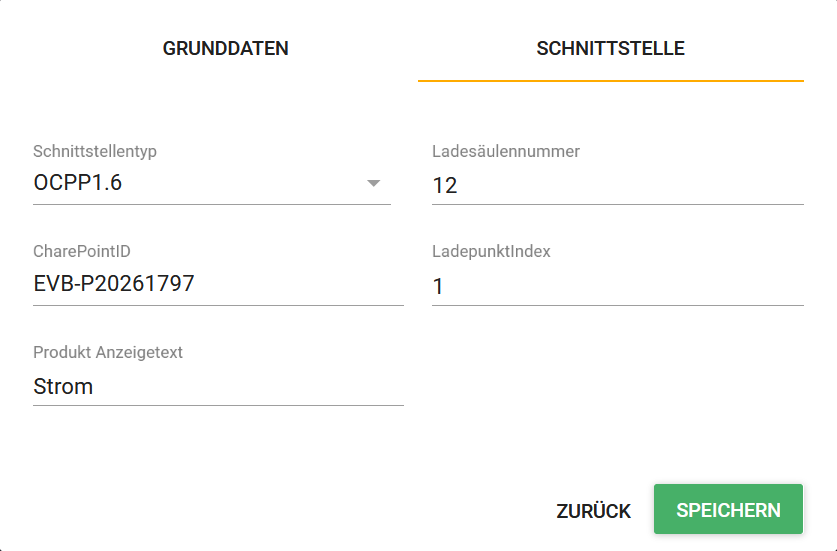
\includegraphics[width=0.75\textwidth]{images/System/Cloud_Schnittstellen_config_charging_stations.PNG}}
	\caption{Erweiterte Stationen Konfiguration für eine Ladesäule in der Cloud Weboberfläche \cite{Kunde_Weboberflaeche}}
	\label{fig:Cloud_Schnittstell_konfig}
\end{figure}

\noindent Die neuen Felder wurden bei der Datenbankerstellung im Code hinzugefügt. Somit sieht die finale Datenbanktabelle wie in \autoref{tab:Dantenbank_Tabelle_Stations_final} dargestellt aus.

\noindent Für die Erweiterung der Weboberfläche wurden die Änderungen an das Partnerunternehmen weitergegeben, dass für die Entwicklung der Cloud Weboberfläche verantwortlich ist und von diesem implementiert. Die Konfiguration einer Ladesäule sieht folglich nun wie in \autoref{fig:Cloud_Schnittstell_konfig} dargestellt aus. Dabei ist die Ladesäulennummer Äquivalent zu der \spverb|chargePointNumber| und der Ladepunktindex Äquivalent zum \spverb|chargePointIndex|.
\begin{table}[H]
	\begin{center}
		\begin{tabular}{|ll|}
			\hline
			\multicolumn{2}{|l|}{\textbf{Stations}}           \\ \hline
			\multicolumn{1}{|l|}{id}                & TEXT    \\ \hline
			\multicolumn{1}{|l|}{number}            & TEXT    \\ \hline
			\multicolumn{1}{|l|}{isLocked}          & INTEGER \\ \hline
			\multicolumn{1}{|l|}{isLockLevelLocked} & INTEGER \\ \hline
			\multicolumn{1}{|l|}{lockLevel}         & INTEGER \\ \hline
			\multicolumn{1}{|l|}{currentLockLevel}  & INTEGER \\ \hline
			\multicolumn{1}{|l|}{limitTransaction}  & INTEGER \\ \hline
			\multicolumn{1}{|l|}{isOnStorage}       & INTEGER \\ \hline
			\multicolumn{1}{|l|}{counter}           & INTEGER \\ \hline
			\multicolumn{1}{|l|}{productId}         & TEXT    \\ \hline
			\multicolumn{1}{|l|}{storageId}         & TEXT    \\ \hline
			\multicolumn{1}{|l|}{hwMode}            & TEXT    \\ \hline
			\multicolumn{1}{|l|}{hwChannel}         & INTEGR  \\ \hline
			\multicolumn{1}{|l|}{type}              & TEXT    \\ \hline
			\multicolumn{1}{|l|}{impulseRate}       & INTEGER \\ \hline
			\multicolumn{1}{|l|}{\textbf{chargePointId}}     & \textbf{TEXT}    \\ \hline
			\multicolumn{1}{|l|}{\textbf{chargePointIndex}}  & \textbf{INTEGER} \\ \hline
			\multicolumn{1}{|l|}{\textbf{chargePointNumber}} & \textbf{INTEGER} \\ \hline
		\end{tabular}
	\end{center}
	\caption{Erweiterte Datenbanktabelle \glqq{}Stations\grqq{} \cite{Eigene_Darstellung}}
	\label{tab:Dantenbank_Tabelle_Stations_final}
\end{table}
\subsection{Lösungsstrategie}
Nachdem geklärt wurde, wie die Ladesäulen identifiziert werden können und der Umfang des Protokolls ermittelt wurde, konnte über das weitere Vorgehen diskutiert werden. Um den Softwareaufbau der Erweiterung festzulegen, wurden im Folgenden die Möglichkeiten durchgegangen, wie das Protokoll integriert werden könnte. Dabei gibt es die Möglichkeit über bereits entwickelte Softwarebibliotheken die benötigten Teile/Komponenten/Funktionen des Protokolls zu ergänzen oder das Protokoll gänzlich selbst in \cpp zu entwickeln.
\subsubsection{Bibliotheken}
Um \acs{OCPP} in die Firmware des Tankautomaten zu integrieren, gibt es mehrere Bibliotheken, die bereits eine volle \acs{OCPP} Umsetzung anbieten. Diese sollen hier kurz beschrieben und anschließend verglichen werden. Für den Vergleich wurden neben \cpp, ebenfalls Java und Python Bibliotheken in die Auswahl aufgenommen. Diese konnten mit einbezogen werden, da es möglich ist Python- oder Java Code in einer anderen Applikation einzubetten (vgl. \cite{Python-embedding, Java-embedding}). Dadurch konnte ein breiteres Spektrum an Bibliotheken miteinbezogen werden. Die gefundenen Bibliotheken sollen im Folgenden vorgestellt, analysiert und bewertet werden. Die Bewertungskriterien waren dabei:
\begin{itemize}
	\item Lizenzbedingungen: ist die Bibliothek kommerziell oder frei nutzbar?
	\item Umfang: Welche OCPP Funktionen, Versionen und Rollen werden unterstützt?
	\item Abhängigkeiten: Werden andere Bibliotheken oder Compiler benötigt?
	\item Dokumentation: Ist dokumentiert, wie die Bibliothek genutzt werden sollte?
	\item Schätzung des Integrationsaufwands: Wie viel Aufwand wird zur Integration benötigt?
	\item Schätzung des Entwicklungsaufwands: Wie viel Aufwand wird zur Entwicklung der Applikation mit der Bibliothek benötigt?
\end{itemize}

\noindent Die Bibliotheken sollen dabei nicht nur untereinander verglichen werden, sondern auch mit einer eigenen Umsetzung des Protokolls.

\begin{table}[H]
	\textbf{\textit{Open-ocpp}}\cite{Open-ocpp}\\
	\begin{tabularx}{\textwidth}{| c | X |}
		\multicolumn{1}{c}{} & \multicolumn{1}{c}{}\\ \hline
		Lizenz & LGPLv2.1  \newline \\
		Umfang & Voller Umfang der Version 1.6. Kann sowohl in der Charge Point oder Central System Rolle genutzt werden.  \newline \\
		Abhängigkeiten & OpenSSL, libwebsockets, SQLite, rapidjson\newline \\
		Sprache & \cpp \\ \hline
	\end{tabularx}
	\caption{\label{tab:test_tabelle} Einordnung der open-ocpp Bibliothek \cite{Eigene_Darstellung}}
\end{table}

\noindent Open-ocpp ist eine aktiv unterstütze Bibliothek für die OCPP Version 1.6, geschrieben in \cpp. Sie ist unter der \acfi{LGPL}-2.1 Lizenziert und damit kommerziell frei nutzbar, solange die Bibliothek für jeden verfügbar bleibt (vgl. \cite{GNU_LGPL2_1}). Sie beinhaltet als Netzwerkstack libwebsockets, speichert Konfigurationen in einer lokalen SQLite Datenbank ab, nutzt zur Verwaltung von TLS Zertifikaten OpenSSL und benutzt rapidjson zur \acs{JSON} Serialisierung/Deserialisierung. Alle \acs{OCPP} Nachrichten der Version 1.6 werden unterstützt und sie kann zur Integration der \acs{CSMS} Rolle oder der Ladesäulen Rolle genutzt werden. Die Bibliothek verwaltet das Versenden und Empfangen der Nachrichten. Der Nutzer muss dabei nur selber Callback Funktionen implementieren, die Daten für das Versenden und Empfangen von Nachrichten, bereitstellen. Die Dokumentation der Bibliothek erfolgt durch Kommentare im Code, Beispiele im Repository und einer Beschreibung des Umfangs.

\begin{table}[H]
	\textbf{\textit{Libocpp}}\cite{Libocpp}\\
	\begin{tabularx}{\textwidth}{| c | X |}
		\multicolumn{1}{c}{} & \multicolumn{1}{c}{}\\ \hline
		Lizenz & Apache 2.0 \newline \\
		Umfang & Unterstützt OCPP v1.6 nur in der Charge Point Rolle\newline \\
		Abhängigkeiten & python3-pip, boost, SQLite, OpenSSL\newline \\
		Sprache & \cpp\\ \hline
	\end{tabularx}
	\caption{\label{tab:test_tabelle} Einordnung der Libocpp Bibliothek \cite{Eigene_Darstellung}}
\end{table}

\noindent Libocpp ist ebenfalls eine in \cpp geschriebene Bibliothek zur Implementierung von \acs{OCPP} 1.6. Da sie allerdings nur zur Integration der Ladesäulen Rolle geeignet ist, sie von der Auswahl ausgeschieden. \\
\begin{table}[H]
	\textbf{\textit{MicroOcpp}}\cite{MicroOcpp}\\
	\begin{tabularx}{\textwidth}{| c | X |}
		\multicolumn{1}{c}{} & \multicolumn{1}{c}{}\\ \hline
		Lizenz & LGPLv2.1\newline \\
		Umfang & Unterstützt OCPP v1.6 nur in der Charge Point Rolle\newline \\
		Abhängigkeiten & OpenSSL, libwebsockets, SQLite, rapidjson, doctests\newline \\
		Sprache & C/\cpp\\ \hline
	\end{tabularx}
	\caption{\label{tab:test_tabelle} Einordnung der MicroOcpp Bibliothek \cite{Eigene_Darstellung}}
\end{table}

\noindent MicroOcpp unterstützt wie LibOcpp nur die Ladesäulen Rolle und ist damit als ungeeignete Bibliothek ausgeschieden. Allerdings bietet MicroOcpp zusätzlich zur Bibliothek einen umfangreichen Simulator an, der eine voll funktionsfähige OCPP 1.6 Ladesäule simulieren kann(vgl. \cite{MicroOcpp-Simulator}). Dieser kann später zu Testzwecken eingesetzt werden (siehe \autoref{Testumgebung}).
\begin{table}[H]
	\textbf{\textit{Mobilityhouse ocpp}} \cite{Mobilityhouse-ocpp}\\
	\begin{tabularx}{\textwidth}{| c | X |}
		\multicolumn{1}{c}{} & \multicolumn{1}{c}{}\\ \hline
		Lizenz & \acs{MIT} Lizenz\newline \\
		Umfang & Unterstützung von OCPP v1.6 - v2.0.1 für \acs{CSMS} und Ladesäulen \newline \\
		Abhängigkeiten & Python 3.12, Package Installer for Python (PIP), Python Websockets \newline \\
		Sprache & Python\\ \hline
	\end{tabularx}
	\caption{\label{tab:test_tabelle} Einordnung der Mobilityhouse-ocpp Bibliothek \cite{Eigene_Darstellung}}
\end{table}

\noindent Die vom deutschen Unternehmen \glqq{}The Mobility House\grqq{} entwickelte OCPP Bibliothek, ist die Umfangreichste zur Auswahl stehende Bibliothek und bietet als einzige eine komplette Lösung für die OCPP Versionen 1.6 bis 2.0.1 an. Sie funktioniert dabei ähnlich wie Open-ocpp und übernimmt das Empfangen, Senden, Verarbeiten und Einordnen der Nachrichten. Über ein Interface können dann Werte gesetzt werden, um auf den Inhalt einer Nachricht zu antworten. Dabei muss die Applikation entscheiden, wie dabei auf eine Nachricht reagiert wird oder wann eine Nachricht versendet wird. Die Bibliothek wird über eine \acfi{MIT} Lizenz vertrieben und kann somit ohne Einschränkungen genutzt werden(vgl. \cite{MIT-Lizenz}). Da die Bibliothek in Python geschrieben ist, bedarf es zur Nutzung der neusten Version der Bibliothek Python 3.12, dem Package Installer von Python (\acfi{PIP}) und der Python WebSockets Bibliothek. Die Dokumentation ist nicht sehr umfangreich und bietet nur, für die jeweilige OCPP Version, ein erklärtes Beispiel zur Instanziierung eines \acs{CSMS} oder einer Ladesäule.
\begin{table}[H]
	\textbf{\textit{Java-OCA-OCPP}}\cite{Java-OCA}\\
	\begin{tabularx}{\textwidth}{| c | X |}
		\multicolumn{1}{c}{} & \multicolumn{1}{c}{}\\ \hline
		Lizenz & MIT-Lizenz\newline \\
		Umfang & Unterstützung von OCPP v1.6 und v2.0 für \acs{CSMS} und Ladesäulen\newline \\
		Abhängigkeiten & Java, Maven, Java-Websocket\newline \\
		Sprache & Java\\ \hline
	\end{tabularx}
	\caption{\label{tab:test_tabelle} Einordnung der Java-OCA-OCPP Bibliothek \cite{Eigene_Darstellung}}
\end{table}

\noindent Die Java-OCA-OCPP Bibliothek ist auf Java basierend und unterstützt neben OCPP Version 1.6 die Version 2.0. Die OCPP Version 2.0 hat im Vergleich zu Version 2.0.1 einige Fehler. Sie ist nicht kompatibel mit der Version 2.0.1 und sollte somit nicht mehr implementiert werden(vgl.\cite{OCPP-2.0.1-part0-introduction}, S.3). Aus diesem Grund kann die Bibliothek maximal zur Implementierung der Version 1.6 genutzt werden. Im Gegensatz zu den vorher beschriebenen Bibliotheken, wird kein direktes Interface geboten um Daten für Nachrichten bereitzustellen. Stattdessen werden hier die Methoden jeder Nachrichten Klasse überschrieben und von der Nutzer Applikation neu implementiert. Dabei muss der Nachrichteninhalt manuell überprüft werden und ein Rückgabewert angegeben werden. Dies bedeutet, dass die Bibliothek nur das Empfangen, Versenden und Einordnen der Nachrichten übernimmt. Die Bibliothek basiert ebenfalls auf der \acs{MIT} Lizenz und ist damit frei einsetzbar. Neben Java wird Maven und die Java-Websocket Bibliothek zum Einsatz benötigt. Die Dokumentation ist aus den bisher gelisteten Bibliotheken, die schwächste. Es gibt keine Beschreibung zum Einsatz der Bibliothek und es ist nur ein rudimentäres Beispiel ohne Kommentare im Repository zu finden. \\
\subsubsection{Eigenlösung}
\begin{table}[H]
	\begin{tabularx}{\textwidth}{| c | X |}
		\multicolumn{1}{c}{} & \multicolumn{1}{c}{}\\ \hline
		Lizenz & Unterliegt der Konzept Informationssysteme GmbH\newline \\
		Umfang & Enthält nur die benötigten Komponenten, die zuvor identifiziert wurden \newline \\
		Abhängigkeiten & WebSocket Bibliothek\newline \\
		Sprache & \cpp\\ \hline
	\end{tabularx}
	\caption{\label{tab:test_tabelle} Einordnung der Selbstentwicklung \cite{Eigene_Darstellung}}
\end{table}
\noindent Bei einer eigenen Implementierung müssen folgende Dinge integriert werden:
\begin{itemize}
	\item Das WebSocket Protokoll, zum unterliegenden Datentransport
	\item Das RPC Protokoll/Framework zum Formatieren der Daten und zur Verwaltung der Nachrichten
	\item Das OCPP Protokoll zum Verarbeiten und erstellen der Nachrichten
\end{itemize}
Sollte die Selbstentwicklung gewählt werden, muss ebenfalls eine Lösung für die WebSocket Kommunikation gefunden werden. Hierfür kann entweder die Qt WebSocketServer Klasse benutzt werden \cite{QWebsocketServer}, oder erneut eine andere geeignete \cpp Bibliothek gesucht werden. \newline

\noindent Der Vorteil ggü. den bereits entwickelten Lösungen ist, dass eine eigene Lösung individueller angepasst werden kann. Darüber hinaus kann diese auch zur einfachen Erweiterung designt werden. Außerdem kann durch die Selbstentwicklung Zeit gespart werden, falls der Umfang dieser nicht sehr groß ist, was hier zu trifft. Dabei muss, aber auch beachtet werden, dass die Selbstentwicklung im Vergleich zu den fertigen Bibliotheken nicht bereits getestet wurde.
\subsubsection{Vergleich}
\noindent Nachdem bereits festgestellt wurde, dass weder LibOcpp noch MicroOcpp zur Integration in die Terminalsoftware geeignet sind, beläuft sich die finale Auswahl der Bibliothek auf: Open-ocpp, Mobilityhouse-ocpp oder Java-OCA-OCPP. Um die Auswahl einzugrenzen werden die Bibliotheken erst untereinander verglichen und danach abgewogen, ob es überhaupt sinnvoll ist diese anstelle einer eigenen Implementierung vorzuziehen. \\

\noindent Im Vergleich zu den beiden anderen Bibliotheken Java-OCA-OCPP dabei am schlechtesten abgeschnitten. Sie bietet keine Vorteile im Bereich Lizenz, Umfang, Dokumentation, Integrationsaufwand oder Entwicklungsaufwand ggü. den anderen beiden Bibliotheken. Deshalb kam sie nicht als zu nutzende Bibliothek infrage.\\

\noindent Im Kriterium Umfang obliegt die Funktionalität von Mobilityhouse-ocpp der von Open-ocpp, da hier bereits beide OCPP Versionen implementiert sind. Da die Terminalsoftware allerdings bereits in \cpp programmiert ist, ist die Open-ocpp Bibliothek einfacher zu integrieren. Der Entwicklungsaufwand mit den Bibliotheken konnte nur schwer bewertet werden, da hier mehrere Faktoren kollidieren. Sollte die Mobilityhouse Bibliothek genutzt werden, entfällt der Aufwand zur Integration einer weiteren OCPP Version. Dafür muss allerdings Python in die Applikation eingebettet werden und für einen Mechanismus gesorgt werden, mit dem die erhaltenen Daten aus Python wieder in der \cpp Applikation genutzt werden können. Außerdem sorgt die Integration von Python in die Applikation, für eine schlechtere Übersicht über die Abläufe der Firmware.\\

\noindent Der Aufwand zur Erweiterung von Open-ocpp um die Protokollversion 2.0.1 ist ebenfalls schwer einzuschätzen. Der Aufwand zur Integration des Daten- und Nachrichtenaustausch entfällt im Vergleich zur Selbstentwicklung. Allerdings ist nicht garantiert, dass die Struktur der Bibliothek eine einfache Erweiterung zulässt.\newline

\noindent Aufgrund der genannten Gegebenheiten wurde deshalb der größere Aufwand in Kauf genommen, um das Protokoll selbst zu entwickeln. Dabei soll dafür das Protokoll so implementiert werden, dass Erweiterungen leicht gestaltbar sind und z. B. auch einfach TLS hinzugefügt werden kann.
\subsubsection{WebSocket Bibliothek}
Da in der Auswahl die Eigenlösung als beste Option angesehen wurde, muss nun wie bereits erwähnt eine geeignete Lösung für die WebSocket Kommunikation gefunden werden. Dabei war die QWebSocketServer Klasse am naheliegendsten. Jedoch wurde sehr schnell klar, dass diese nicht genutzt werden kann. Dies lag daran, dass in der genutzten Qt Version 5.15LTS, die QWebSocketServer Klasse keine Unterstützung für WebSocket Subprotokolle anbietet (vgl. \cite{QWebsocketServer}, \glqq{}Detailed Desription\grqq{}). Diese sind allerdings unverzichtbar, wie bereits in \autoref{OCPP_Websockets} dargelegt. Daher musste erneut nach einer zusätzlichen Bibliothek gesucht werden. \newline
\noindent Diesmal wurde sich jedoch ausschließlich auf \cpp Bibliotheken beschränkt, da nicht \cpp Bibliotheken für die WebSocket Kommunikation dieselben Nachteile mit sich bringen wie die bereits vorgestellten OCPP Bibliotheken. Dabei wurden ausschließlich Bibliotheken ausgesucht, die ein hohes Abstraktionslevel bieten, um die Entwicklungs- und Einarbeitungszeit einzugrenzen. Es wurde ebenfalls darauf geachtet, dass die Bibliotheken WebSocket Subprotokolle und TLS unterstützen, um später eventuelle Erweiterungen zu ermöglichen. Dies schränkte die Anzahl an infrage kommenden Bibliotheken stark ein. Weswegen nur noch zwei zur Auswahl standen: Boost.beast\cite{Boost-beast} und  WebSocketpp\cite{Websocketpp}. Boost.Beast basiert allerdings auf der extrem großen und umfangreichen Boost Bibliothek. Da ansonsten beide Bibliotheken aber gleichermaßen die benötigten Funktionalitäten beinhalten, wurde sich aufgrund des kleineren Umfangs für die Websocketpp Bibliothek entschieden.

\subsection{Geplantes Vorgehen}
Da nach der Auswahl geklärt wurde, welche Bibliotheken zum Einsatz kommen sollen, konnte für die Erweiterung ein geeignetes Vorgehen geplant werden. Dabei wurde die beste Reihenfolge ermittelt und mithilfe der diskutierten Anforderungen eine geeignete Lösung entworfen.
\subsubsection{Modifikation der bestehenden Systeme}
Im ersten Schritt sollen bereits bestehende Funktionen, an die neue Schnittstelle angeglichen werden. Dafür müssen Klassen und Methoden angepasst werden, damit zwischen der bestehenden Impulsschnittstelle und OCPP unterschieden werden kann. Da dieser Schritt die Grundlage für alle weiteren Funktionen ist, muss dieser vor allen anderen Schritten erledigt werden.
\subsubsection{GUI Planung}
Als Nächstes kann die GUI angepasst werden. 
Zur Erweiterung der GUI wurde sich an den Anforderungen T-01 bis T-09 orientiert. Um die dort beschriebenen Prozesse zu realisieren, muss die neue Stationsauswahl für Ladesäulen angezeigt werden, nachdem in der Produktauswahl die \glqq{}E-Ladestationen\grqq{} Option ausgewählt wurde. In \autoref{fig:Modifizierter_Ablauf_GUI} ist der geplante Ablauf mit dieser Modifikation zusehen.
\begin{figure}[H]
	\centering
	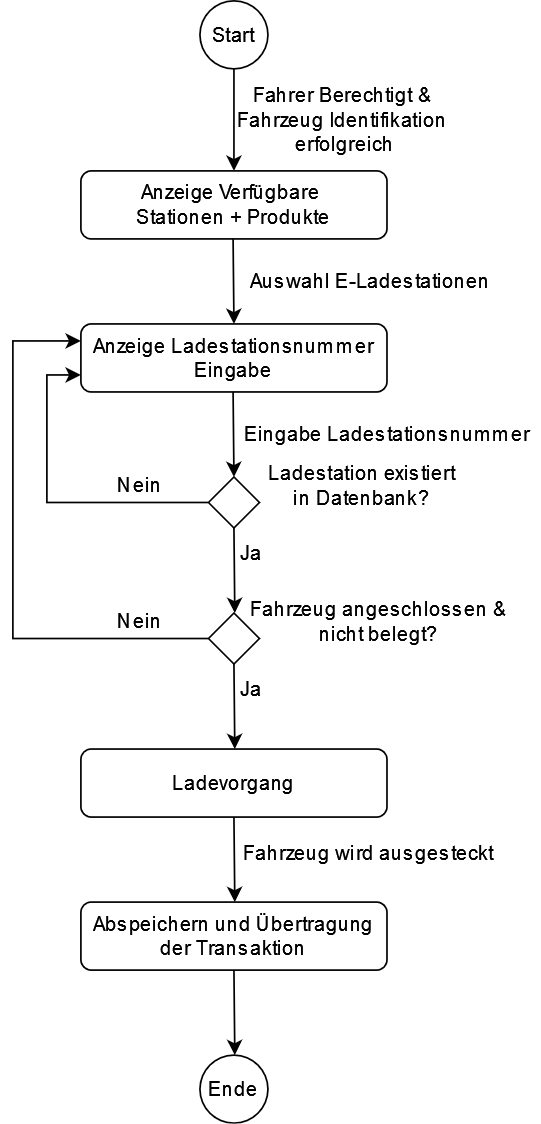
\includegraphics[width=0.35\textwidth]{images/Architektur/Ablauf_Ladevorgang(1).png}
	\caption{Ablauf mit erweiterter GUI \cite{Eigene_Darstellung}}
	\label{fig:Modifizierter_Ablauf_GUI}
\end{figure}

\noindent Um die Fehlermeldungen zu realisieren, muss der Status der Ladesäule geprüft werden. Hierfür kann der übermittelte Status in der \spverb|StatusNotification|/\spverb|TransactionEvent| Nachricht genutzt werden. Basierend auf dem Status kann daraufhin entweder der Ladevorgang gestartet werden, oder eine Fehlermeldung erscheint in der Stationsauswahl. Wird der Ladevorgang gestartet und der Ablauf ist identisch zu einer normalen Tankung. \\

\noindent Neben diesem muss auch ein Sonderverhalten implementiert werden, das auftritt, sobald ein Fahrer/Fahrzeug nur für eine Ladesäule freigegeben ist oder insgesamt nur eine Ladesäule mit dem Tankautomaten verbunden ist. Dieser Fall ist in \autoref{fig:Abaluf_eine_Station} zu sehen. Sollte einer dieser Fälle eintreten, muss die Auswahl übersprungen werden und direkt ein Ladevorgang gestartet werden. Im Fehlerfall soll dabei die Produktauswahl geöffnet werden, in der nur die verbundene Ladesäule zusehen ist. Die Fehlermeldung soll in der Produktauswahl angezeigt werden. Sobald der Fehler behoben ist, kann dann nach der Auswahl der Station in der Produktauswahl, wieder die Stationsauswahl geöffnet werden. Über die erneut ein Ladevorgang gestartet werden kann. 
\begin{figure}[H]
	\centering
	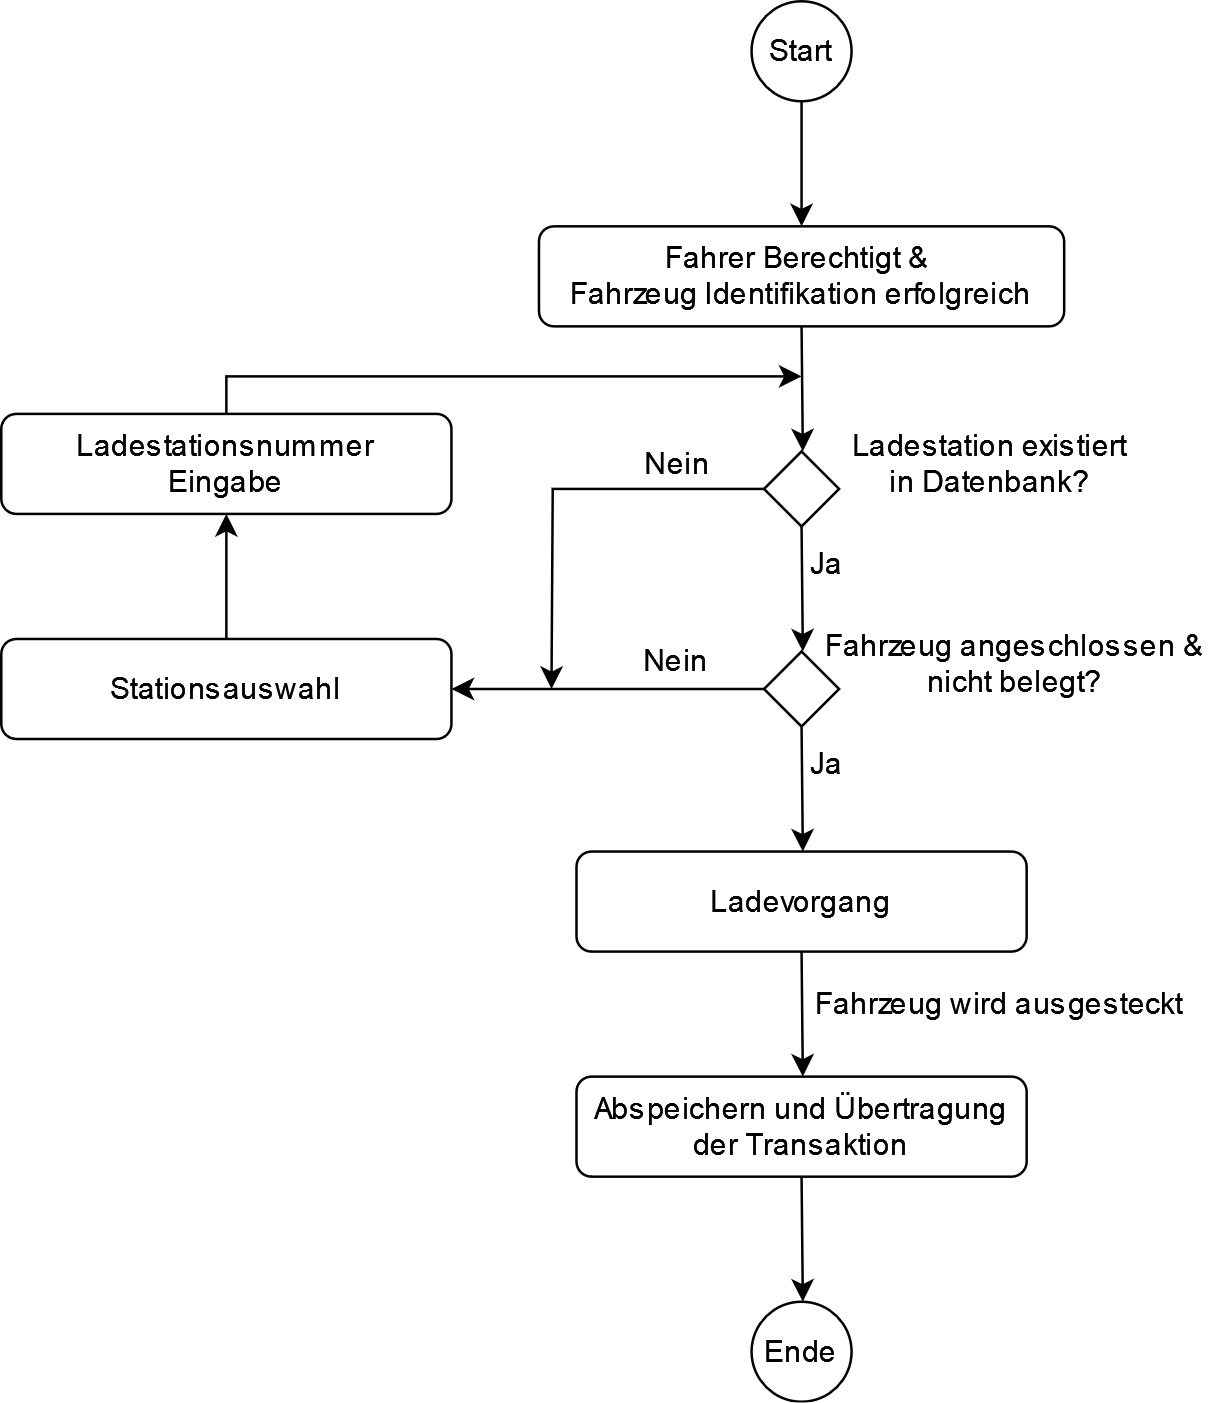
\includegraphics[width=0.6\textwidth]{images/Architektur/Ablauf_eine_Station.jpg}
	\caption{Ablauf bei nur einer Verbundenen oder freigegebenen Ladesäule \cite{Eigene_Darstellung}}
	\label{fig:Abaluf_eine_Station}
\end{figure}
\subsubsection{Integration von OCPP}
Als vorletzten Schritt soll das Protokoll implementiert werden. Da das Protokoll aus mehreren Ebenen besteht, kann sich beim Vorgehen an diesen orientiert werden. Konkret ist damit gemeint, dass zuerst die WebSocket Kommunikation integriert wird. Auf dieser basiert das RPC Protokoll, das als nächstes integriert wird. Am Schluss wird dann das eigentliche OCPP Protokoll eingebunden und die benötigten Nachrichtentypen hinzugefügt. Zuerst soll die Protokollversion 1.6 eingebunden werden und danach ergänzend die Version 2.0.1. Da für OCPP 1.6 weitaus mehr Testmöglichkeiten durch z. B. Simulatoren bestehen und die Interaktion mit der Ladesäule hier unkomplizierter ist, wurde sich für dieses Vorgehen entschieden. Wie diese Komponenten aufgebaut werden, wird in \autoref{OCPP_Architektur} beschrieben.

\subsubsection{Cloud Schnittstellen Erweiterung}
Im letzten Schritt sollen die Cloud Anforderungen umgesetzt werden. Um die Anforderung C-01 zu erfüllen, kann der bereits vorhandene Mechanismus zur Synchronisation zwischen Terminal und Cloud genutzt werden. Hierbei kann anhand der \spverb|Heartbeat| Nachricht erkannt werden, ob eine Ladesäule noch online ist und mit dem Terminal kommuniziert. Dieser Status kann über ein \spverb|bool| Wert mit der Cloud synchronisiert werden und wird ebenfalls alle 60s mit den anderen Daten aktualisiert. Für die Anforderung C-02, gibt es keine Schritte, die konkret erfolgen müssen, da ein Ladevorgang analog zu einem Tankvorgang behandelt werden sollte. Falls irgendwelche unerwarteten Fehler auftreten, werden diese während der Umsetzung gelöst werden müssen. 

\subsection{Architektur der Schnittstelle}\label{OCPP_Architektur}
Da sich die OCPP Schnittstelle auf keine bereits existierenden Strukturen stützt, musste für diese eine eigene Architektur ausgearbeitet werden. Dabei wurden die Zusammenhänge der Schnittstelle analysiert und ein Konzept entwickelt, wie die Strukturen untereinander und mit der restlichen Applikation interagieren können.
\subsubsection{Komponenten Aufbau}
Um eine Übersicht zu schaffen, wie die Integration des Protokolls aussehen soll, wurde hierfür das Modell in \autoref{fig:Komponenten_Aufbau} aufgebaut. Hier werden die einzelnen Komponenten als Blackbox dargestellt und deren Zusammenhang erklärt. Hier ist unwichtig, wie die Komponenten im inneren Funktionieren. Stattdessen soll die Funktion der Komponenten und deren Interaktionen mit anderen Komponenten im Fokus stehen. Der geplante Entwurf besteht aus drei Komponenten, die jeweils für die Verwaltung unterschiedlicher Schichten des Protokolls verantwortlich sind. Der WebSocketServer soll auf WebSocketpp aufbauen und die Verbindungen zu den Ladesäulen managen. Das RPC Framework soll das Versenden und Empfangen der drei unterschiedlichen RPC Nachrichtentypen verwalten. Zusätzlich soll es Nachrichten im RPC Format ent- und verpacken. Im OCPP Handler soll der Inhalt von empfangenen Nachrichten gespeichert werden und der Inhalt für zu versendende Nachrichten bestimmt werden. Es soll für beide OCPP Versionen jeweils ein Handler existieren, um die beiden Versionen besser zu trennen und um eine Überschneidung gleichnamiger Nachrichtentypen zu vermeiden. Beide sollen aber dasselbe Verhalten aufweisen.\newline

\begin{figure}[H]
	\centering
	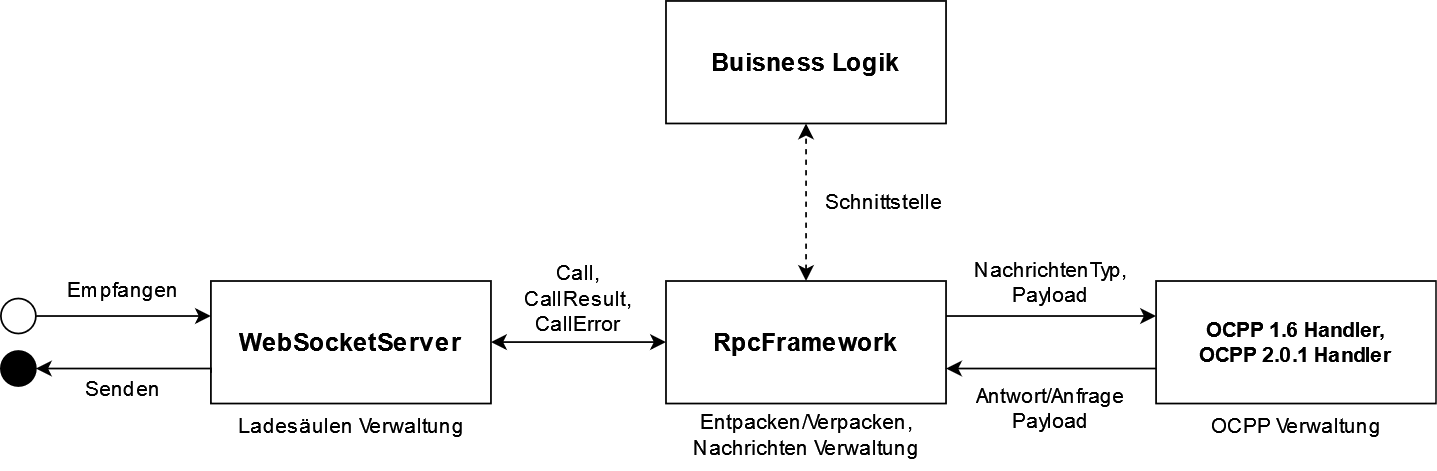
\includegraphics[width=1.0\textwidth]{images/Architektur/Zusammenhang_Module.png}
	\caption{Komponenten Ansicht zum geplanten Softwareaufbau der Schnittstelle\cite{Eigene_Darstellung}}
	\label{fig:Komponenten_Aufbau}
\end{figure}

\noindent Als Schnittstelle zur restlichen Programmlogik soll das RPC Framework dienen, da dieses sowohl Zugriff auf den WebSocketServer als auch auf die OCPP Nachrichten Verwaltung hat. Somit kann anhand restlicher Programmabläufe eine OCPP Nachricht versendet werden und auch zum Beispiel beim Empfangen einer Nachricht die restliche Programmlogik darauf reagieren.

\noindent Die Komponenten sollen dabei jeweils die benötigten Bestandteile austauschen, um ihre Funktion zu erfüllen. Der WebSocketServer tauscht mit dem RPC Framework also immer komplette Nachrichten als String aus. Zwischen dem OCPP Handler und dem RPC Framework wird ein OCPP Nachrichtentyp und ein JSON Payload ausgetauscht. \\
\noindent Dadurch können dieselben Strukturen für die unterschiedlichen Abläufe beim Empfangen und Versenden von Nachrichten genutzt werden. Eine Kombination ist dabei ebenfalls sehr einfach. 

\subsubsection{Threads}
Beim bisherigen Stand der Applikation wurden alle Events nur von einem Thread verarbeitet. Um die Applikationseingaben nicht zu stören, soll die Nachrichtenverarbeitung/Erstellung in einem neuen Thread laufen. Der Vorteil von diesem Vorgehen ist, dass die Applikation dadurch sehr schnell alle OCPP Nachrichten, versenden und beantworten kann. Außerdem kann somit der Server dynamisch aktiviert und deaktiviert werden, da der Thread einfach beendet werden kann, wenn z. B. keine Ladesäulen konfiguriert wurden. Bei der Umsetzung muss aber dementsprechend darauf geachtet werden, dass keine \textit{Deadlocks} oder \textit{Race Conditions} dabei entstehen. Damit dies ohne großen Aufwand möglich ist, können zur Kommunikation zwischen den beiden Threads der \textit{Signals and Slots} Mechanismus genutzt werden. Diese sind Thread sicher (vgl. \cite{Qt-signals-and-slots}), helfen der Übersicht und können Dank dem geplanten Event basierten Ablauf gut integriert werden.
\subsubsection{OCPP Nachrichten Struktur}
Um die OCPP Schnittstelle möglichst einfach erweiterbar zu gestalten, sollen die unterschiedlichen Nachrichtentypen gleich aufgebaut sein. Hierfür sollen alle Nachrichten als eine eigene Klasse entworfen werden. Da alle Nachrichten sich anders verhalten, aber immer entweder als eine Anfrage oder Antwort agieren, kann eine Oberklasse definiert werden, von der alle Nachrichten Klassen erben. Somit ist eine gute Übersicht vorhanden, andere Entwickler können direkt erkennen welche Methoden benötigt werden und es ist einheitlich. Ein Beispiel wie dies Aussehen kann ist in \autoref{fig:Nachrichten_Aufbau} zusehen.
\begin{figure}[H]
	\centering
	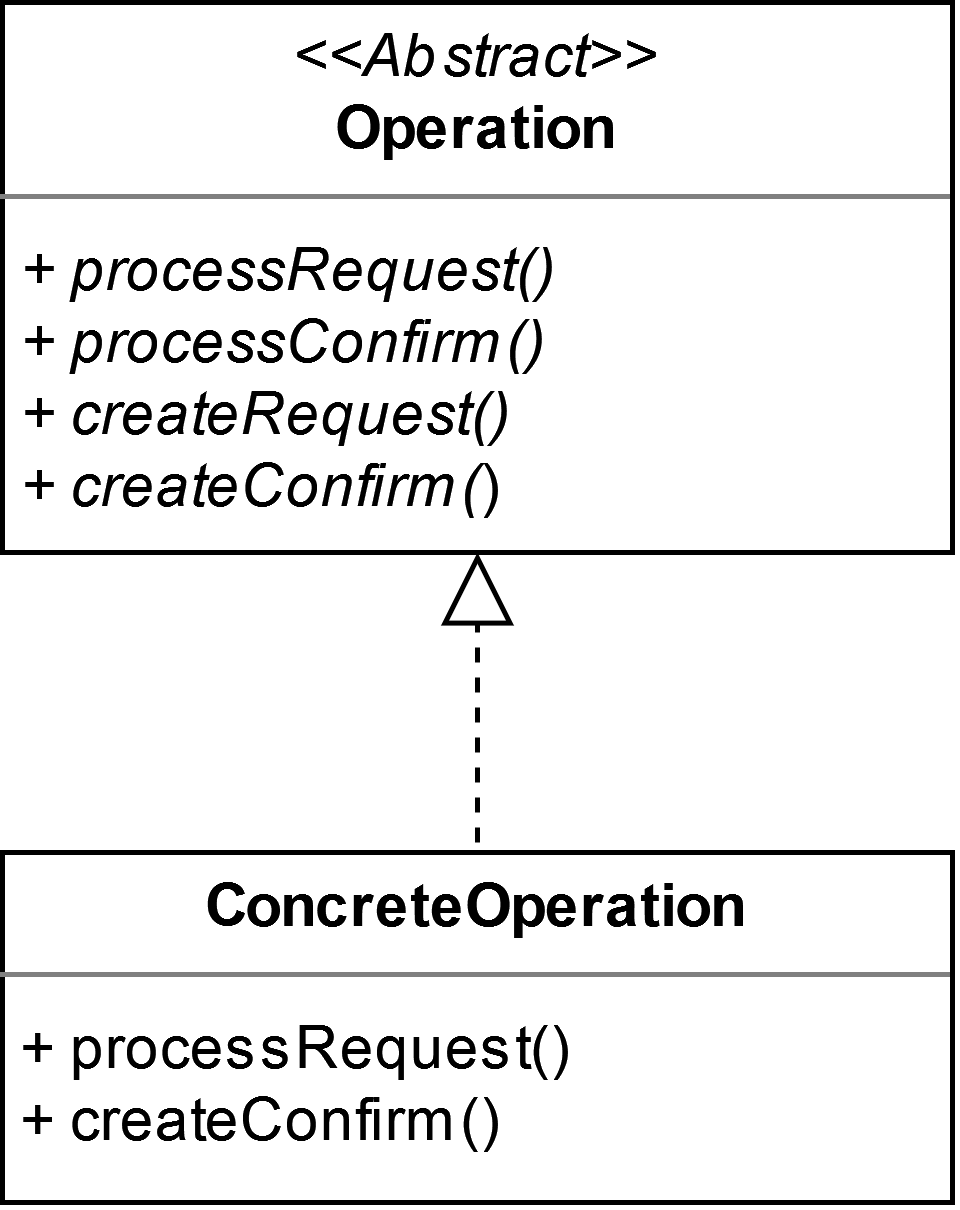
\includegraphics[width=0.3\textwidth]{images/Architektur/Nachrichten_Aufbau.png}
	\caption{Klassendiagramm Darstellung des Nachrichtenaufbau\cite{Eigene_Darstellung}}
	\label{fig:Nachrichten_Aufbau}
\end{figure}
\noindent Dabei sollen Nachrichten jeweils eine Methode zum Erstellen- und zum Verarbeiten einer Antwort/Anfrage besitzen. Somit können die Daten zum Verarbeiten aus dem erhaltenem JSON Payload entnommen werden und in den privaten Membervariablen des Objektes gespeichert werden. Andersherum kann auf Basis der Werte innerhalb des Objektes ein entsprechender JSON Payload erstellt werden. Auf Membervariablen soll dabei mit \spverb|getter|- und \spverb|setter| Methoden zugegriffen werden, damit die Objekte voneinander abgekapselt bleiben können.
\subsubsection{OCPP Nachrichten Handler}
Um die Erweiterbarkeit der Nachrichten zu nutzen, sollen die OCPP Nachrichten über einen Message Handler Aufbau verwaltet werden. Dabei kann aufgrund des Nachrichtentypen unterschieden werden, welche Aktion durchgeführt werden soll. Hierbei müssen alle in \autoref{OCPP_Nachrcihten_bnoetigt} ermittelten Nachrichten als eigene Klasse in der beschriebenen Struktur hinzugefügt werden. Das Ganze kann z. B. als ein \spverb|switch-case| aufgebaut sein, in dem pro Nachrichtentyp ein \spverb|case| existiert. In diesem kann dann lokal ein Nachrichtenobjekt angelegt werden, mit dem die Nachrichten Parameter einfach zu verwalten sind.
